
\documentclass[11pt,a4paper]{article}

\usepackage[utf8]{inputenc} 
\usepackage[T1]{fontenc} 
\usepackage{lmodern}
\usepackage{tcolorbox}

\usepackage[german]{babel}


\setlength{\parindent}{0pt}
\setlength{\parskip}{1ex plus 0.5ex minus 0.5ex}

\usepackage{amsmath} 


\usepackage{graphicx} 

\usepackage[section]{placeins}
\usepackage{booktabs}


\usepackage{hyperref}
\hypersetup{
	colorlinks,
	citecolor=red,
	filecolor=black,
	linkcolor=black,
	urlcolor=black}
\graphicspath{}

\begin{document}
	

{
	\centering 
	\large 
	Physiklabor für Anfänger*innen \\
	Ferienpraktikum im Sommersemester 2018 \\[4mm]
	\textbf{\LARGE 
		Versuch 70: Linsen und Linsensysteme
	} \\[3mm]
	(durchgeführt am 26.09.2018 bei ) \\
	Ye Joon Kim, Marouan Zouari\\
	\today \\[10mm]
}
\tableofcontents

\section{Einleitung}
Mit einer Linse kann man durch die Brechung Licht ablenken. Jede (richtig hergestellte) Linse besitzen zwei Brennpunkte, wo alle parallelen und zur Linse senkrecht einfallenden Lichtstrahlen sich sammeln. Der Abstand von dem Mittelpunkt der Linse zu einem Brennpunkt heißt die Brennweite. Für dicke Linsen und Linsensysteme muss einen weiteren Begriff eingeführt werden. Die doppelte Brechung lassen sich durch Hauptebenen beschreiben. Zwischen den Hauptebenen können die Lichtstrahlen als parallel verlaufend gedacht. Diese Begriffe vereinfachen Berechnungen mit Lichtstrahlen. 

Es existieren mehrere Verfahren, um die Brennweite von Linsen und Linsensysteme zu bestimmen. Bei einer Einzellinse kann die Brennweite $f$ so ausgedruckt werden: 

\begin{equation}
\frac{1}{f} = \frac{1}{g} + \frac{1}{b}
\end{equation}
Wobei $g$ und $b$ die Gegenstandsweite bzw. Bildweite, die Abstände von jeweils dem Gegenstand und Bild zur Linsenmitte, sind.
Für ein Linsensystem, das aus zwei Linsen besteht, gilt eine andere Formel, nämlich:
\begin{equation}
\frac{1}{f} = \frac{1}{f_1}+\frac{1}{f_2}-\frac{d}{f_1f_2}
\end{equation}
Wobei $f_1$ und $f_2$ die Brennweiten der einzelnen Linsen und $d$ der Abstand dazwischen sind. 

Aber wenn die Hauptebenen nicht bekannt sind, können $g$ und $b$ nicht direkt bestimmt werden. In diesem Fall hilft das Bessel-Verfahren, wobei die Brennweite mit:
\begin{equation}
f = \frac{s^2-e^2}{4s}
\end{equation}
bestimmt werden kann, wobei $s$ der Abstand zwischen dem Gegenstand und Bild, und $e$ die Differenz der Positionen, wo Abbildungen möglich sind. 

Mit einem anderen Verfahren, lassen sich die Brennweite und die Hauptebenen gleichzeitig bestimmen, dieses Verfahren heißt das Abbe-Verfahren. Für das Abbe-Verfahren wird einen Punkt ausgewählt und im Referenz zu diesem Punkt die scheinbare Gegenstandsweite $g'$ und die scheinbare Bildweite $b'$ gemessen. Hier wird außerdem der Abbildungsmaßstab verwendet: 
$$ \beta = \frac{B}{G} = \frac{b}{g}$$
Wobei $B$ und $G$ jeweils de Größen des Bildes und Gegenstands sind. 
Mit direkten Messungen von $B$, $G$, $g'$ und $b'$ kann mit den Gleichungen:
\begin{equation}
\begin{array}{l}
	g' = (1+\frac{1}{\beta})\cdot f_1 + h_1 \\
	b' = (1+\beta)\cdot f_2 + h_2
\end{array}
\end{equation}
die $f$ und $h$ bestimmt werden, da $f$ die Steigungen, und $h$ den Achsenabschnitte entsprechen. 



\section{Aufbau und Durchführung}



\section{Auswertung und Fehleranalyse}
Die Werte für $\frac{1}{b}$ wurden gegen $\frac{1}{g}$ aufgetragen. Für jede Messreihe wurde auch lineare Regressionen durchgeführt, aber nur, um die Linearität der Zusammenhang zu veranschaulichen.
\begin{figure}
	\centering
	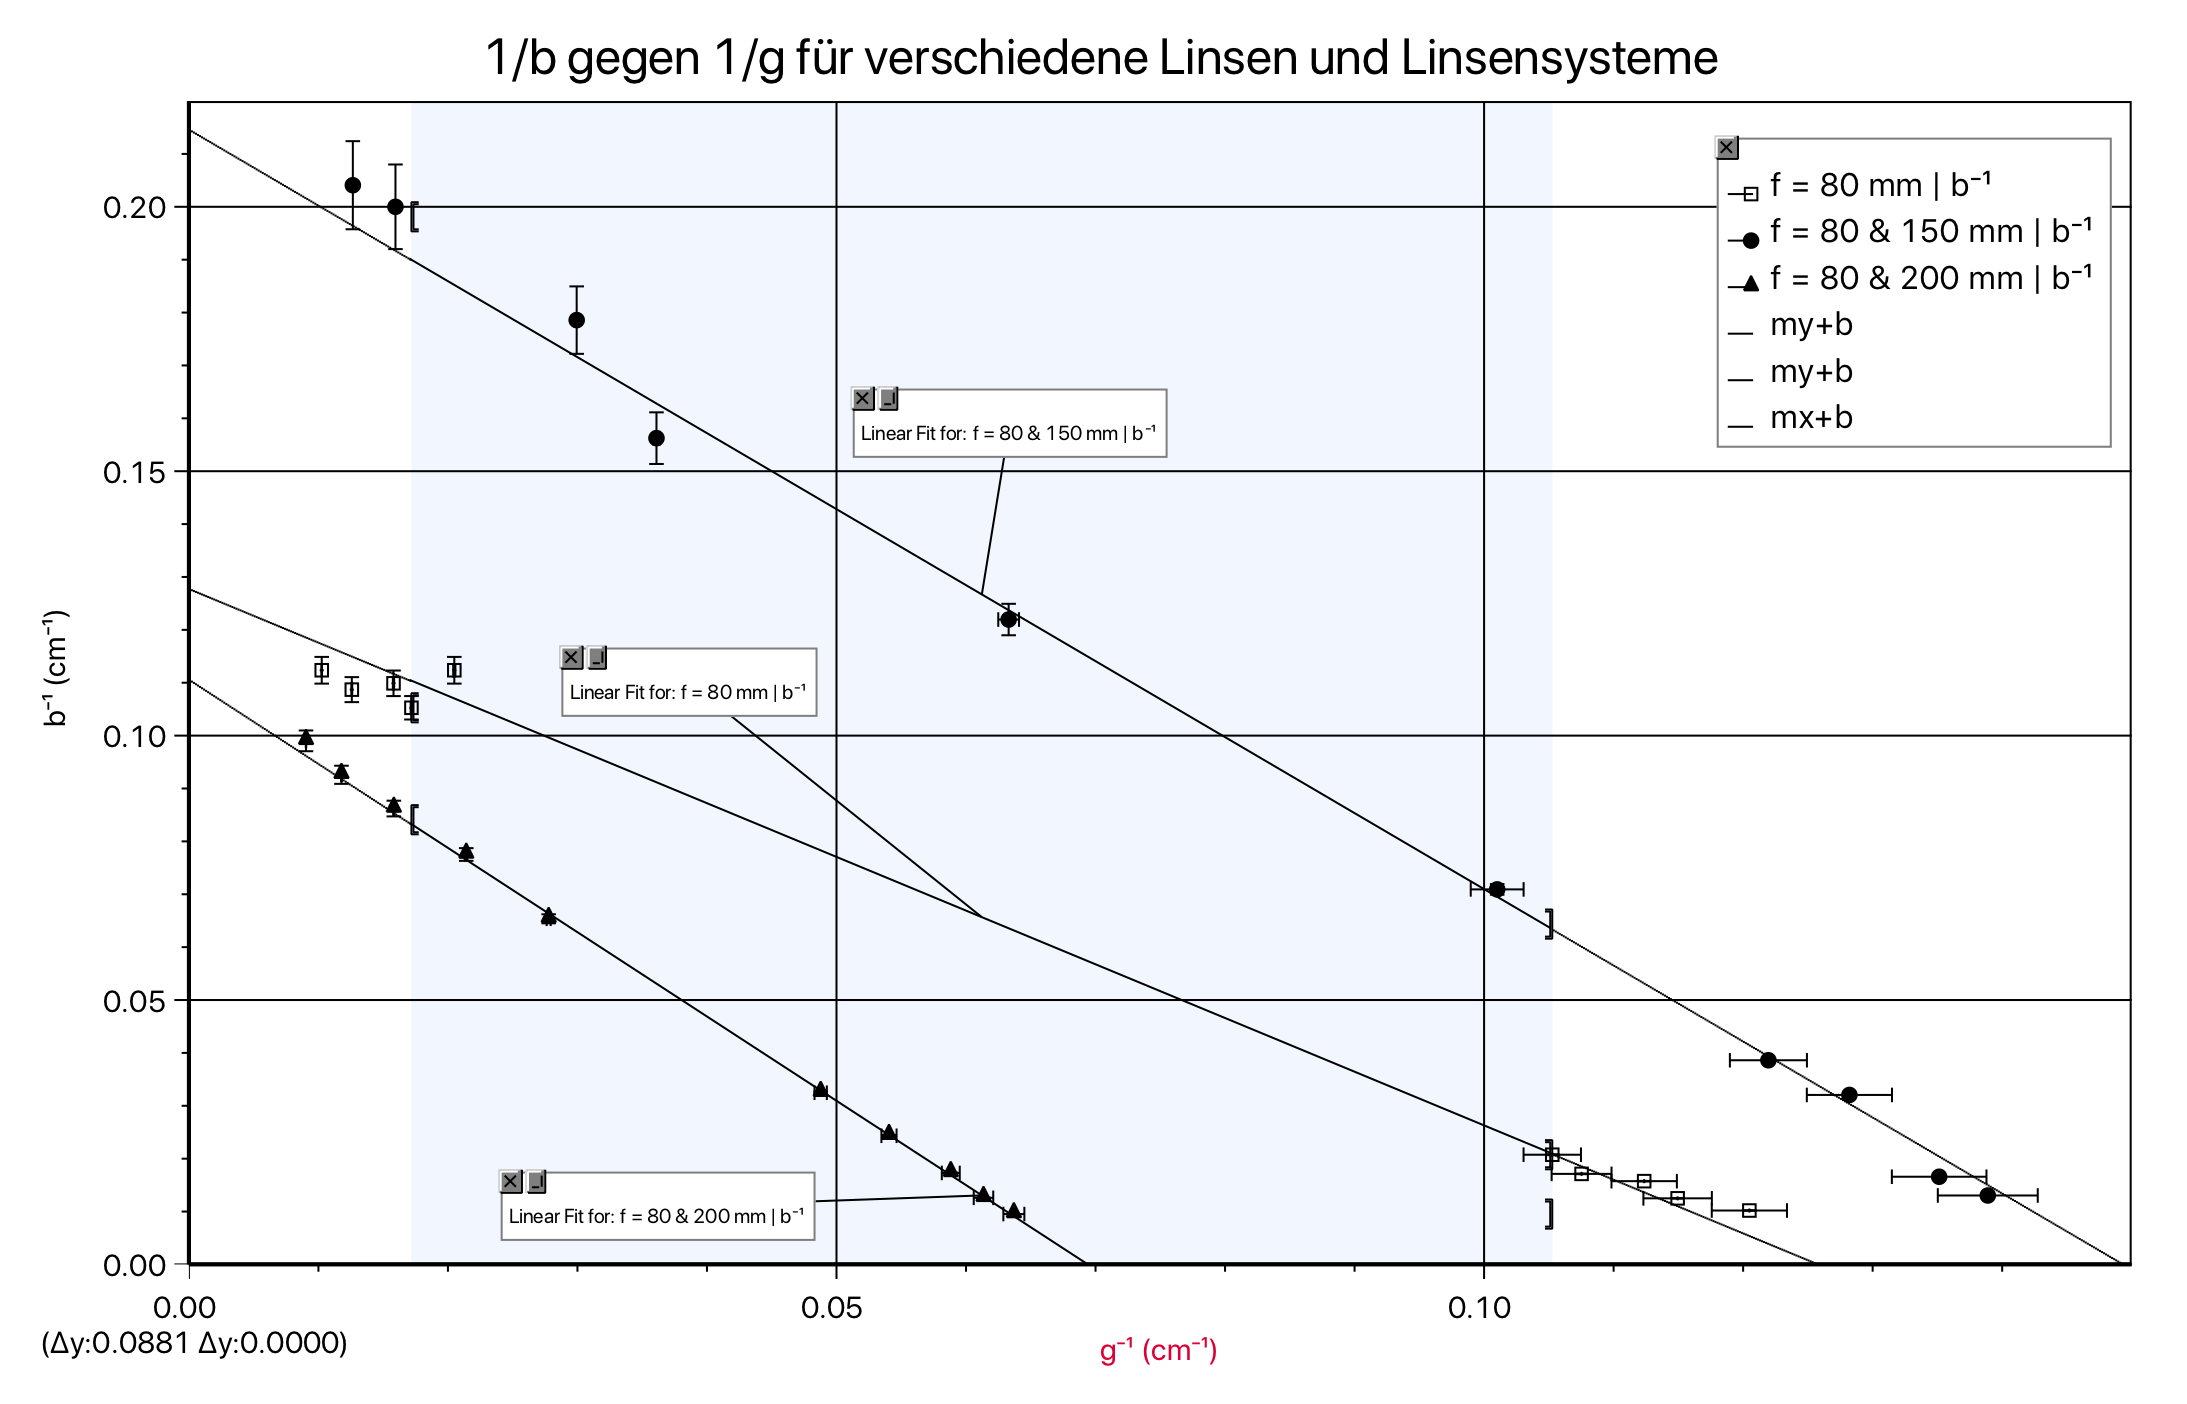
\includegraphics[width=\linewidth]{Abb2}
	\caption{$\frac{1}{b}$ gegen $\frac{1}{g}$.}
\end{figure} 



\section{Diskussion der Ergebnisse}

\section{Anhang}



\end{document}